%第3章

\section{基本設計}

システムの構造を論理的,静的にみるために以下の図\ref{class}に示すクラス図を作成した.

\begin{figure}[htbp]
\centering
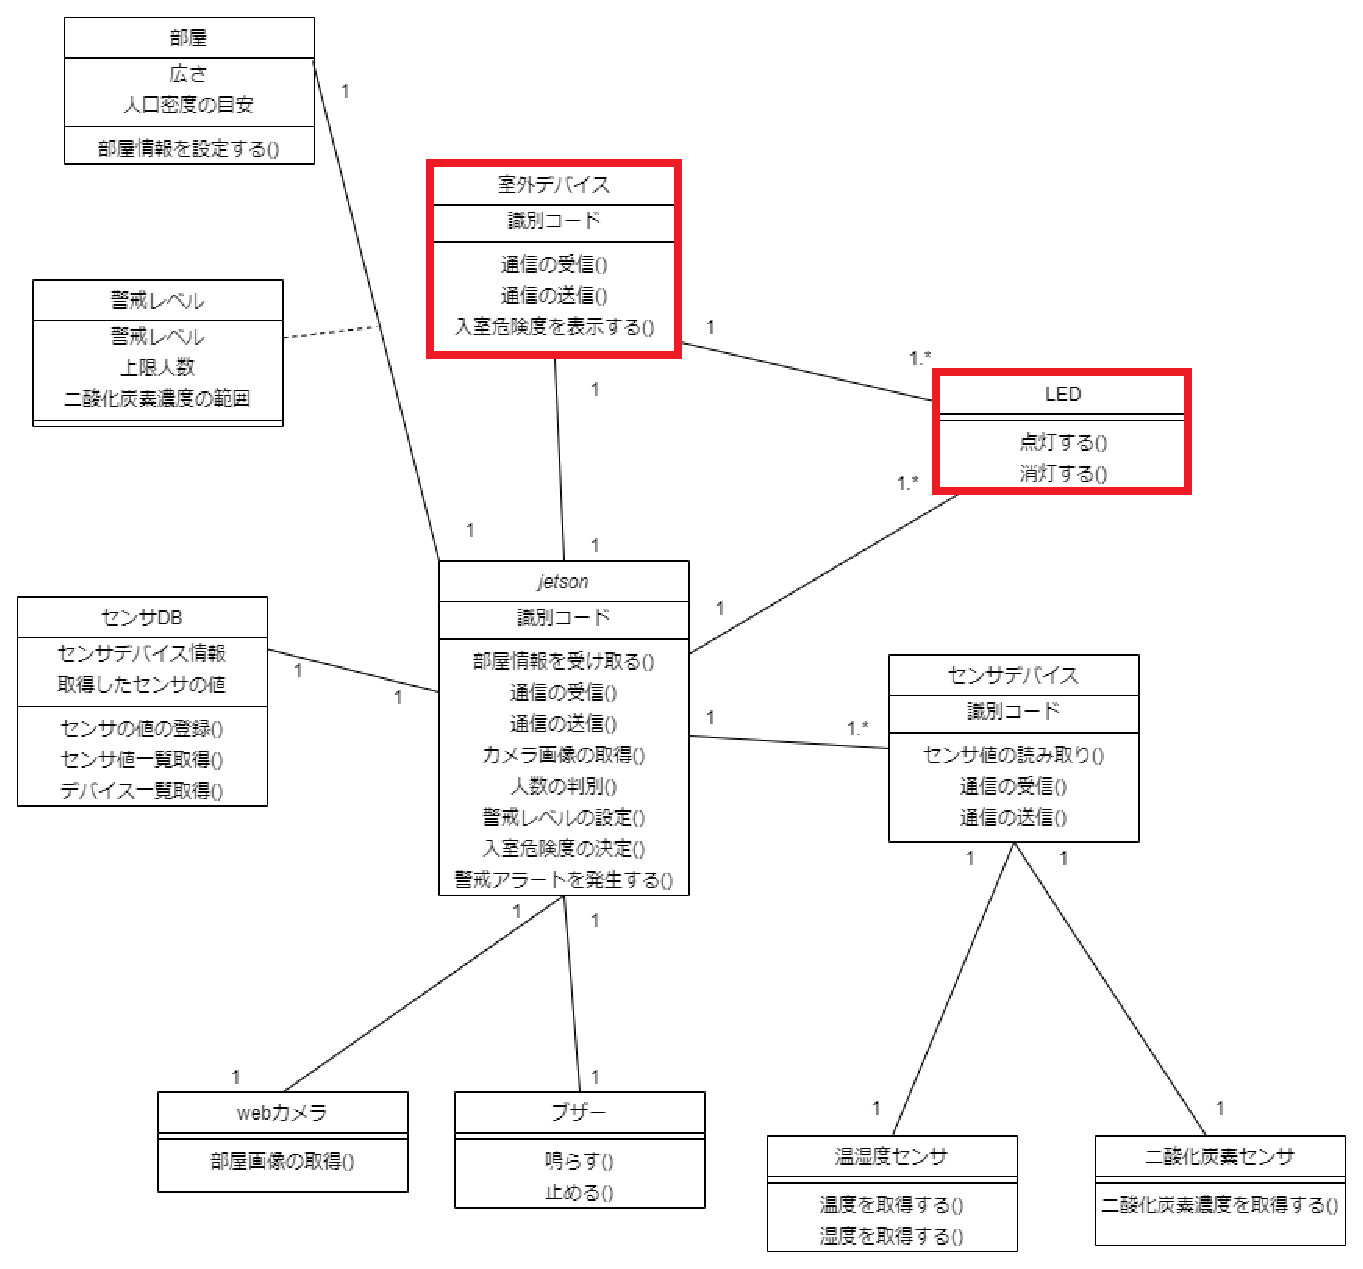
\includegraphics[width=15cm]{./uml/class_e.eps}
\caption{システムのクラス図}
\label{class}
\end{figure}

システムの構成要素として,まずデータ処理等を行うJetsonクラスがある.Jetson一つに対し,室外デバイス,Webカメラ,ブザーがそれぞれ一つずつ存在し,部屋情報クラス,センサデータベースクラス,警戒レベルクラスと関連する.Jetson一つに対しセンサデバイスは複数存在し,センサデバイスは,温湿度センサと二酸化炭素センサをそれぞれ一つずつ持つ.
赤枠で囲んだ室外デバイスとLEDについては筆者が実装する部分となる.
室外デバイスはJetsonと通信するための識別コードがあり,通信の送受信,入室危険度の表示をLEDを用いて行う.

次にユースケースの処理の流れを示すアクティビティ図を作成した.換気要請の受け取りについてのアクティビティ図を図\ref{activitykanki}に,室内環境の監視についてのアクティビティ図を図\ref{activitykanshi}に,入室危険度の確認についてのアクティビティ図を図\ref{activityshitsunai}に示す.

\begin{figure}
	\centering
	\includegraphics[width=0.6\linewidth]{uml/activity_kanki_1}
	\caption{換気要請の受け取りについてのアクティビティ図}
	\label{activitykanki}
\end{figure}

\begin{figure}
	\centering
	\includegraphics[width=0.6\linewidth]{uml/activity_kanshi_1}
	\caption{室内環境の監視についてのアクティビティ図}
	\label{activitykanshi}
\end{figure}

\begin{figure}
	\centering
	\includegraphics[width=0.6\linewidth]{uml/activity_nyushitsu_e}
	\caption{入室危険度の確認についてのアクティビティ図}
	\label{activitynyushitsu}
\end{figure}

\begin{figure}
	\centering
	\includegraphics[width=0.6\linewidth]{uml/activity_shitsunai_2}
	\caption{室内環境の表示についてのアクティビティ図}
	\label{activityshitsunai}
\end{figure}

「換気要請の受け取り」,「室内環境の監視」,「入室危険度の確認」については,3分経過ごとに,センサデバイスが読みだした二酸化炭素濃度をJetsonが受信・記録し,室内の人数推定を行うまでは同じ流れとなる.

「換気要請の受け取り」については,LEDとブザーによる換気要請を出す場合と出さない場合の条件を示している.室内滞在人数が滞在上限人数の75\%を超えている場合,二酸化炭素濃度が15分間連続して基準値を超えていれば換気要請を出し,基準値を超えていなければ換気要請のLEDを消灯させる.室内滞在人数が滞在上限人数の75\%を超えていない場合は,二酸化炭素濃度が上限値を超えていれば換気要請を出し,上限値を超えていなければ換気要請のLEDを消灯させる.

「室内環境の監視」については,警戒レベルの設定についての流れを示している.室内滞在人数が滞在上限人数の75\%を超えている場合,二酸化炭素濃度が15分間連続して基準値を超えていれば警戒レベルを上げ,逆に二酸化炭素濃度が15分間連続して基準値を下回っていれば警戒レベルを下げ,それ以外の場合は何もしない.

「入室危険度の確認」については,室内滞在人数が規定人数を超えている場合,入室危険度を「赤」とし,室内滞在人数が規定人数を超えていない場合は,滞在推奨人数を超えるか否かで分岐する.滞在人数が滞在推奨人数を超えている場合,入室危険度を「赤」とし,超えていない場合は,滞在推奨人数を下回らなければ入室危険度を「黄」,滞在推奨人数を下回っていれば入室危険度を「青」とする.ここで入室危険度について,「赤」は感染リスクが高まっており人数調整が必要な状態,「黄」は現在の滞在人数ならば維持できる状態,「青」は感染リスクを高めない範囲で人数を増やすことができる状態を示す.定めた入室危険度をJetsonから室外デバイスへ送信し,室外デバイスは入室危険度に応じた色のLEDを点灯させる.赤枠で囲んだ室外表示デバイスの動作については筆者が実装を担当する.

「室内環境の表示」については,3分経過ごとにセンサデバイスが読みだした温湿度をJetsonが受信し,温湿度が適正範囲外の場合は室内のLEDが点灯することで警告する.

以上の基本設計より表\ref{ketugoutestkoumoku}に示す結合テスト項目を挙げた.

\begin{table}
	\centering
	\caption{結合テスト項目}
	\label{ketugoutestkoumoku}
	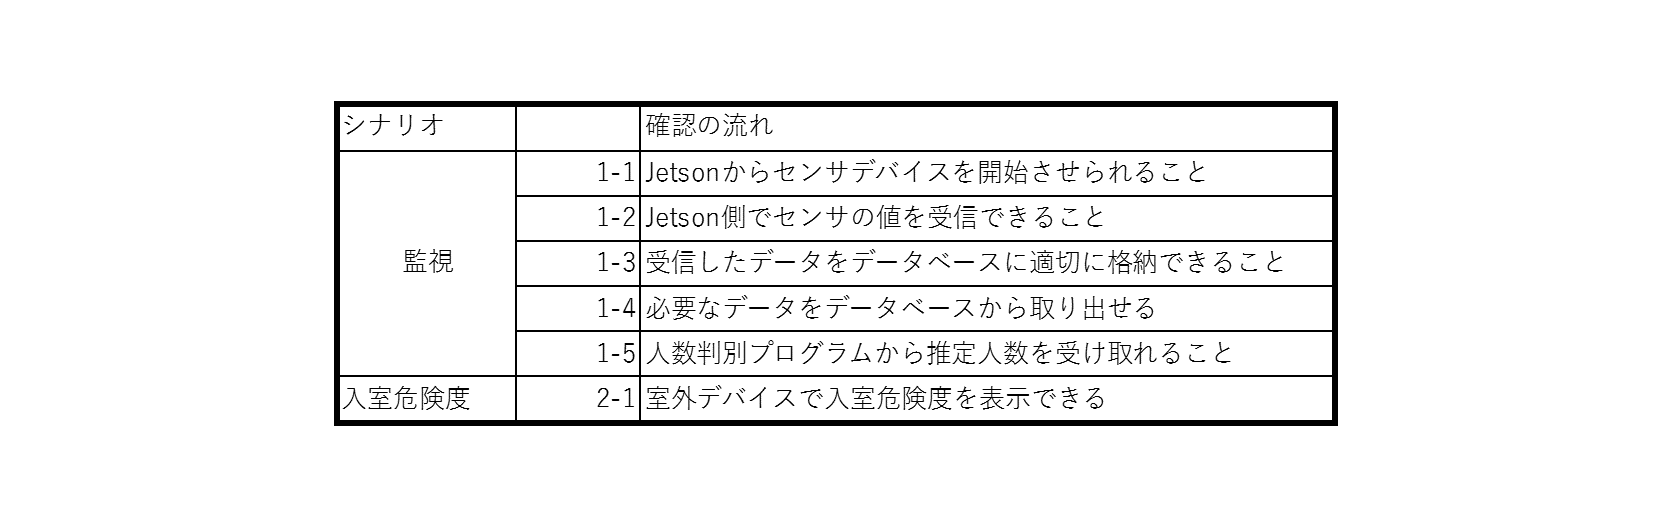
\includegraphics[width=0.9\linewidth]{test/ketugoutest_koumoku}
\end{table}
